\section{Discussion and Error Analysis}
\label{sec:discussion}

\subsection{Why LoRA Outperforms Full Fine-Tuning in Robustness}
Our empirical findings in Section~\ref{sec:experiments} establish that parameter-efficient adaptation via LoRA incurs substantially lower relative degradation under orthographic perturbation (4.68\%) than full fine-tuning (7.01\%). We attribute this resilience to two primary mechanisms:

\subsubsection{Constrained Gradient Manifolds and Overfitting Mitigation}
In full fine-tuning, all 278 million parameters of XLM-RoBERTa are updated. When exposed to a training corpus containing specific canonical spelling realizations, full backpropagation allows weights in early attention and embedding layers to over-specialize to exact surface forms. In contrast, LoRA freezes the underlying representations ($W_0$) and restricts all adaptation to rank-$r$ bottleneck matrices ($r=16$). This constraint prevents catastrophic perturbation of the pre-trained multilingual manifold. When an unseen spelling variant appears during inference, the frozen base model maps the subword composition into a semantically coherent region of the latent space, preserving contextual sentiment cues.

\subsubsection{Subword Tokenization Geometries}
Our subword fertility analysis reveals a nuanced picture. While XLM-RoBERTa's larger SentencePiece vocabulary (250K tokens) yields fewer absolute subwords per canonical word (2.28 vs.\ 2.47 for mBERT's WordPiece), the proportional fragmentation increase under spelling perturbation is slightly higher for XLM-RoBERTa (27.5\% of pairs exhibit increased fragmentation, mean increase of $+0.17$ tokens) compared to mBERT (24.3\%, mean $+0.12$). This indicates that tokenization geometry alone does not explain LoRA's robustness advantage. Rather, the constrained gradient manifold described above is the primary mechanism: by preventing catastrophic perturbation of the pre-trained multilingual representations, LoRA maintains robust inference even when subword decomposition shifts.

\subsection{Why XLM-RoBERTa (Full FT) Underperforms mBERT}
A notable finding is that fully fine-tuned XLM-RoBERTa achieves lower clean accuracy (0.4856) than both mBERT (0.5791) and even TF-IDF (0.5445). We attribute this to \textit{catastrophic forgetting} during full fine-tuning: when all 278M parameters are unconstrained, the larger model is more prone to overfitting the relatively small training set ($N=16{,}420$). The XLM-RoBERTa encoder, pre-trained on 2.5TB of CommonCrawl data across 100 languages, has deeply distributed multilingual representations that are disrupted more severely by unconstrained gradient updates on a narrow Roman Urdu corpus. In contrast, LoRA adaptation preserves these representations and achieves substantially better performance (0.5220 accuracy), confirming that \textit{how} a model is adapted matters more than model capacity alone.

\subsection{Confusion Matrix and Error Boundary Shifts}
To investigate the qualitative failure modes induced by orthographic noise, we examined confusion matrices across Clean and Severe conditions (Fig.~\ref{fig:cm_comparison}).

\begin{figure}[htbp]
\centering
\begin{minipage}{0.48\columnwidth}
    \centering
    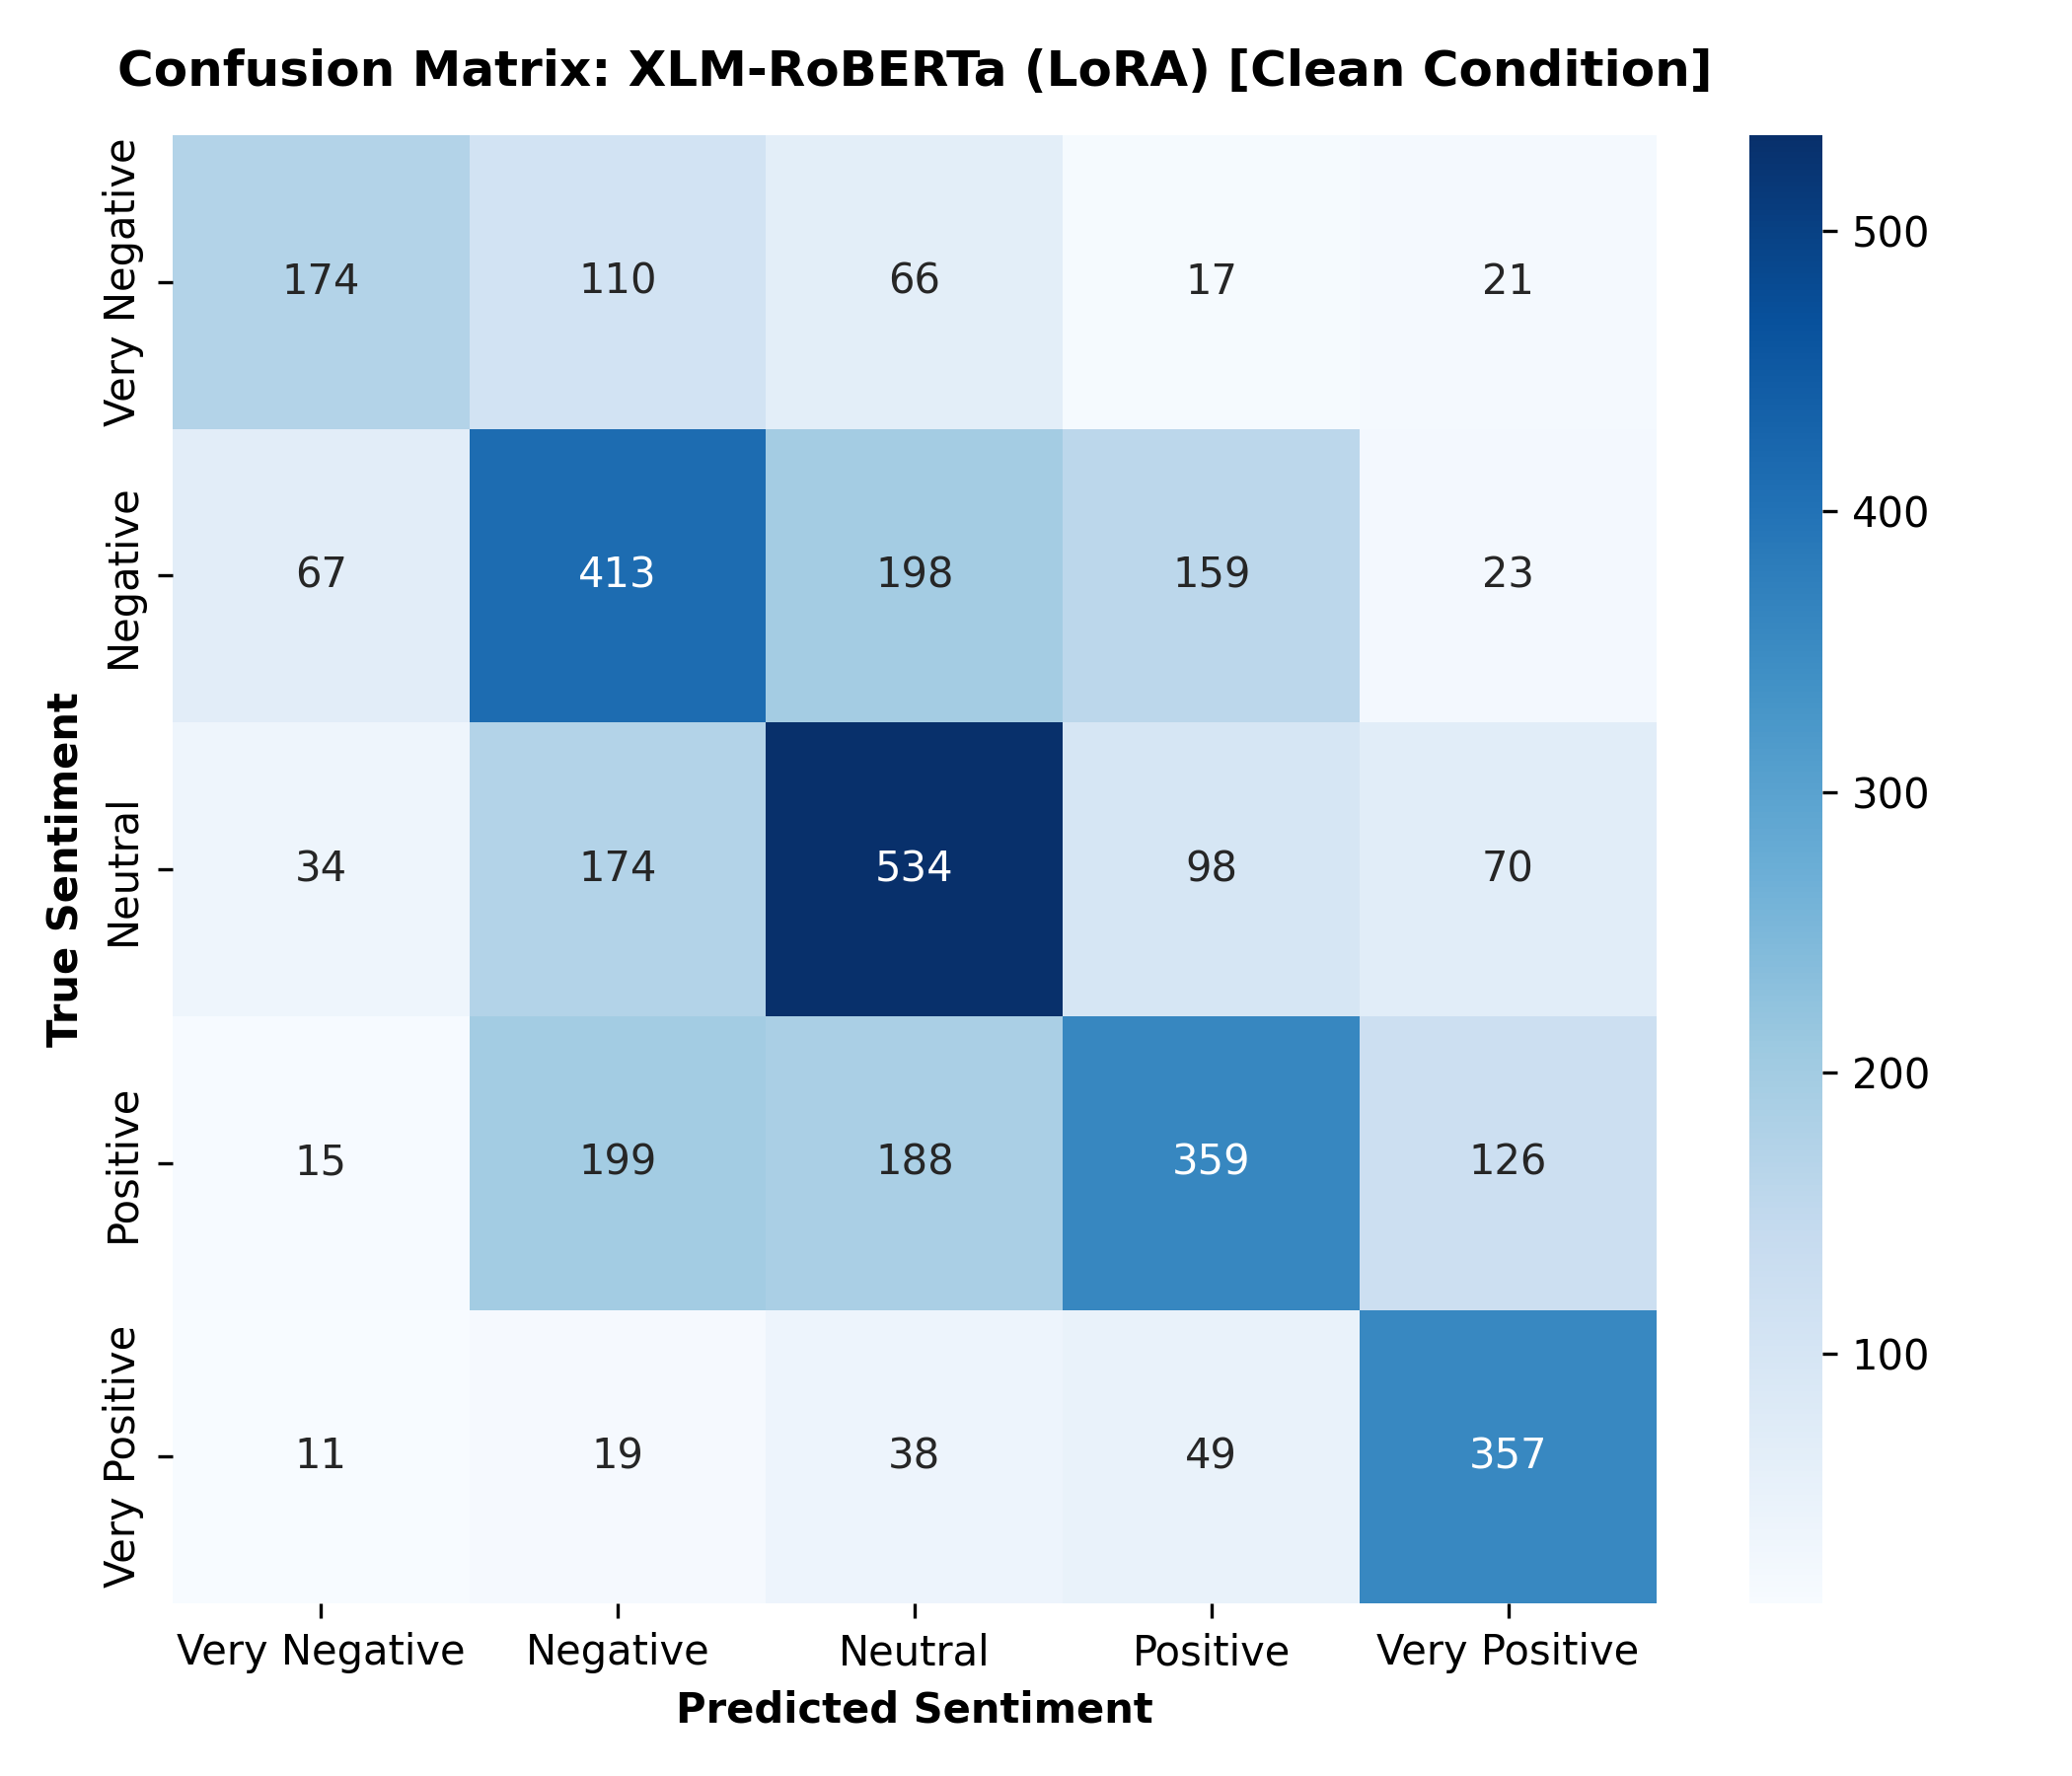
\includegraphics[width=\linewidth]{figures/cm_xlm_roberta_lora_clean.png}
    \centerline{\footnotesize (a) LoRA (Clean)}
\end{minipage}\hfill
\begin{minipage}{0.48\columnwidth}
    \centering
    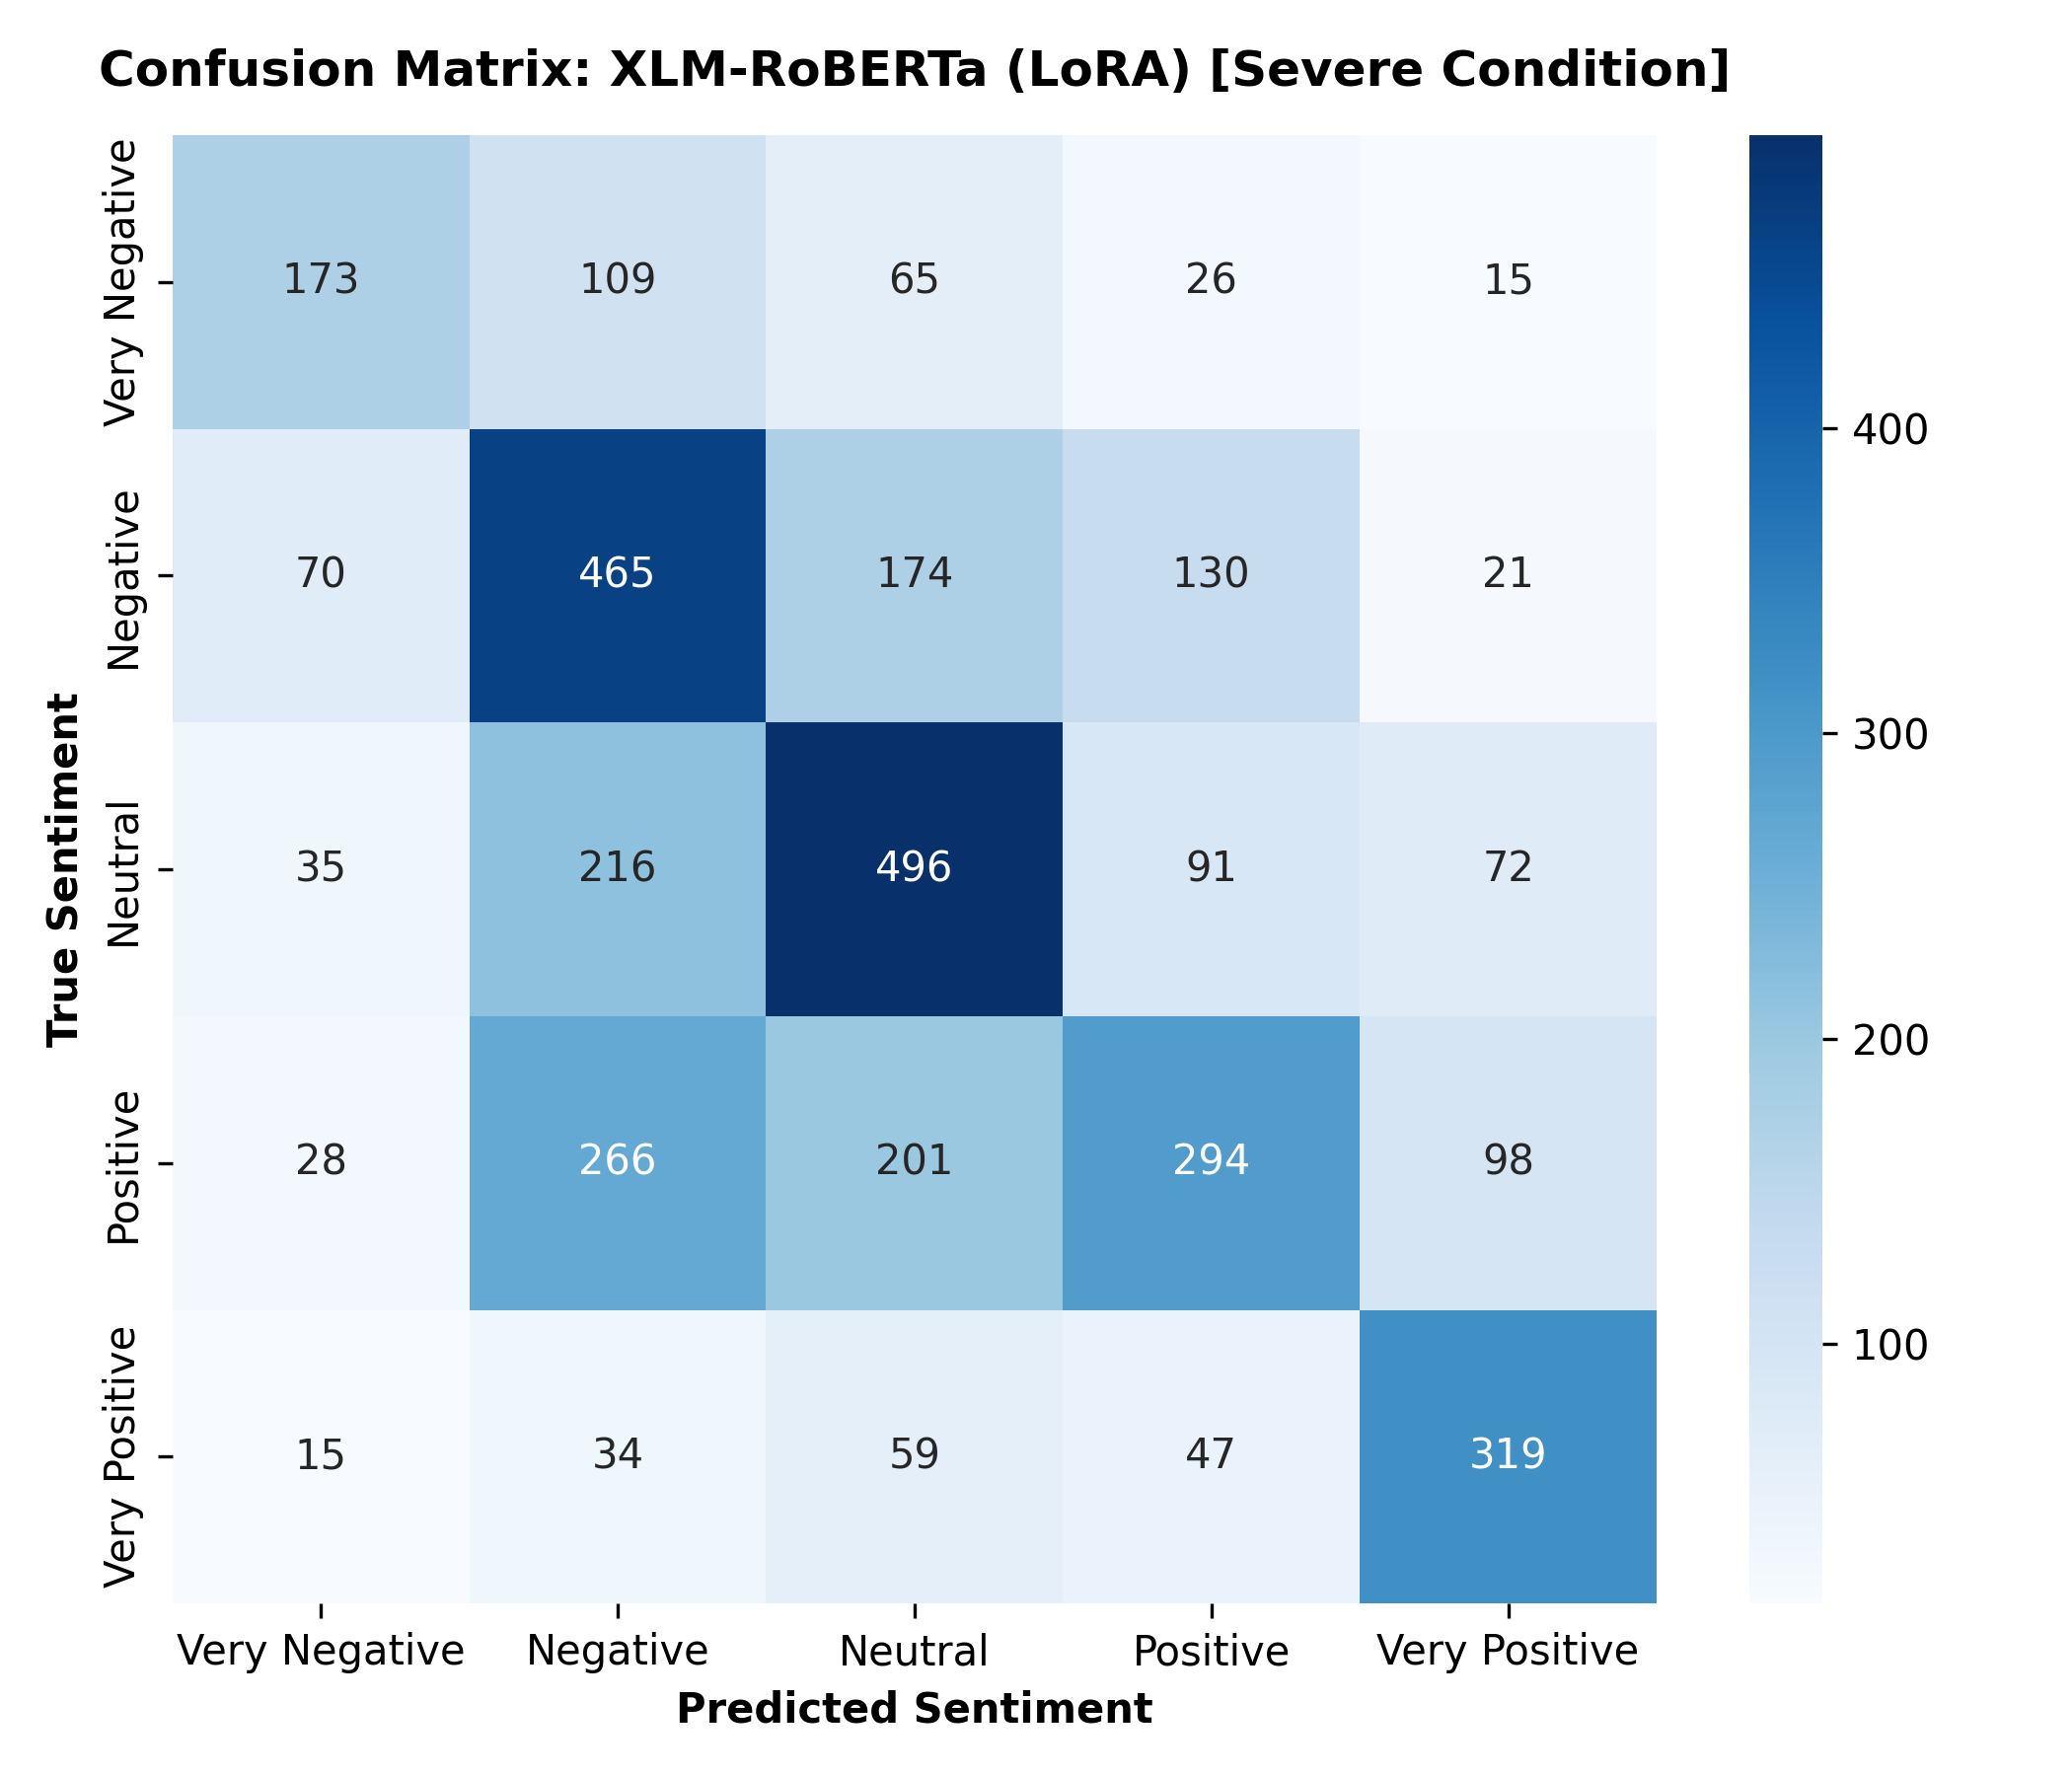
\includegraphics[width=\linewidth]{figures/cm_xlm_roberta_lora_severe.png}
    \centerline{\footnotesize (b) LoRA (Severe)}
\end{minipage}
\caption{Confusion matrices for XLM-RoBERTa (LoRA) on Clean vs. Severe test sets. Severe noise drives systematic regression to the neutral class.}
\label{fig:cm_comparison}
\end{figure}

The error analysis reveals three prominent patterns:
\begin{enumerate}
    \item \textbf{Regression to the Neutral Class:} Under severe orthographic perturbation, misclassifications do not scatter randomly across polarities. Instead, both \textit{Positive} and \textit{Negative} predictions migrate systematically into the \textit{Neutral} class. When sentiment-bearing tokens (e.g., \textit{bohat}, \textit{bura}, \textit{zabardast}) are fragmented into unfamiliar subwords, the attention heads downweight their salience, causing the classifier to default to the uninformative neutral prior.
    \item \textbf{Extreme Polarity Boundary Blurring:} The separation between extreme classes (\textit{Very Positive} vs. \textit{Positive}, and \textit{Very Negative} vs. \textit{Negative}) degrades most rapidly. Modifiers and intensifiers (e.g., \textit{nihayat}, \textit{intehai}) are especially sensitive to spelling corruption, collapsing extreme predictions into moderate categories.
    \item \textbf{Negation Inversion Failures:} A critical failure mode involves negated phrases (e.g., \textit{acha nahi tha} $\rightarrow$ \textit{acha nhn thaa}). Corruption of short function words like \textit{nhn} causes the model to miss the negation operator entirely, inverting predicted sentiment from Negative to Positive.
\end{enumerate}

\subsection{Practical Implications for Industry NLP}
Our results yield direct, actionable guidelines for deploying sentiment analysis systems in low-resource, non-standardized scripts:
\begin{itemize}
    \item \textbf{Abandon Generic Preprocessing:} Standard text normalization routines (stripping emojis, punctuation, and stopwords) yield zero recovery.
    \item \textbf{Adopt Lexicon-Driven Normalization:} Inverting human-curated variant dictionaries recovers over 84\%--93\% of performance loss with negligible computational latency.
    \item \textbf{Prioritize LoRA Over Full Fine-Tuning:} For deployment on edge or cloud servers, LoRA slashes GPU memory footprints by 40\% and significantly improves out-of-distribution robustness.
\end{itemize}

\subsection{Limitations}
Several limitations should be acknowledged. First, all experiments use a single dataset family (RUWV-NSR) with cross-domain validation limited to one additional corpus (RUECD); broader evaluation across social media, SMS, and conversational datasets would strengthen generalizability claims. Second, LoRA was tested with a single rank configuration ($r=16$); a hyperparameter sweep across ranks and target modules could reveal further optimization opportunities. Third, the study evaluates only base-sized transformers ($\leq$278M parameters); emerging large language models and instruction-tuned variants may exhibit different robustness profiles. Fourth, our five-class sentiment taxonomy necessarily reduces per-class sample sizes, contributing to the relatively modest absolute accuracies ($\approx$52--58\%) observed across all models. Finally, we did not compare against other PEFT methods such as QLoRA~\cite{dettmers2023qlora}, AdaLoRA, or prefix tuning, which may offer complementary advantages.
